\setlength{\parindent}{2em} %首行缩进

\section*{實驗目的:}

\begin{enumerate}[label=\arabic*.]
  \item 透過 SDS-PAGE 電泳分析蛋白質分子量
\end{enumerate}

\section*{實驗原理:}

\subsection{聚丙烯醯胺膠体電泳}
\begin{enumerate}
  \item 膠體成分
  \begin{enumerate}[label=\alph*.]
    \item 丙烯醯胺(acrylamide,單體分子)
    \begin{itemize}[]
      \item[-] 具有神經毒性,須戴手套、避免吸入。
      \item[-]  構成孔洞分離物質,acrylamide 濃度越高則孔洞越小。
    \end{itemize}

    \item Bis-acrylamide (架橋分子)
    \begin{itemize}[]
      \item[-] 可看作兩個丙烯醯胺單體分子連結,形成分叉點,幫助膠體聚合。
      \item[-] 和 Acrylamide 一樣具有神經毒性。
    \end{itemize}
    \item ammonium persulfate(APS,自由基)
    \begin{itemize}[]
      \item[-] 產生自由基啟動膠體聚合反映。
    \end{itemize}
    \item tetramethylethylenediamine(TEMED,催化劑)
    \begin{itemize}[]
      \item[-] 幫助自由基傳遞 
    \end{itemize}
  \end{enumerate}

  \begin{center}
    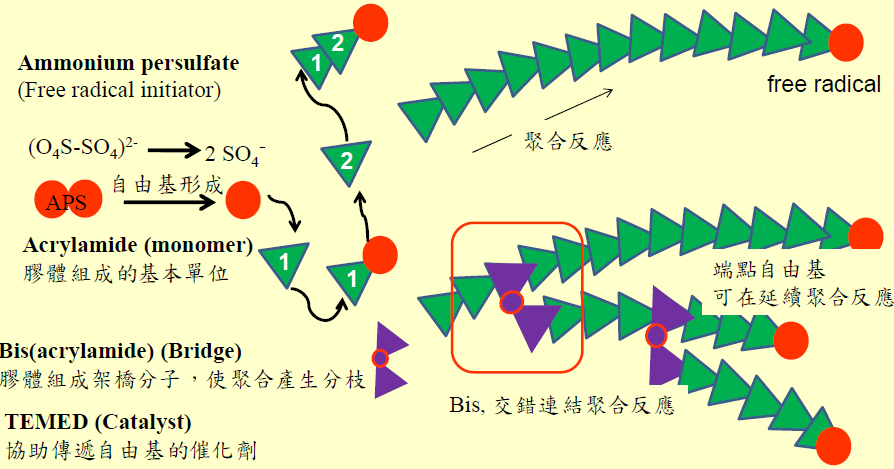
\includegraphics[width=.7\textwidth]{paste_src/2023-11-13-16-17-57.png}
  \end{center}

  \item 梯度電泳系統
  






  \begin{enumerate}[label=\alph*.]
    \item Stacking Gel 功能\\
    \qquad Stacking gel 保證電泳時所有待測物在相同起跑點。樣品為鹼性環境(pH8.3),待測蛋白、Glycine 與 \ce{Cl^-} 都帶負電。通電後因為 Stacking gel 是酸性環境(pH6.9),Gly 轉為電中性阻礙待測蛋白前進,最終 \ce{Cl^-}和Gly會把待測蛋白壓在同一條起跑線。
  \end{enumerate}

  \begin{figure}[H]
    \begin{minipage}[h]{0.6\textwidth} %minipage寬
      \begin{tabular}{cccc}
        \toprule
        名稱  &pH &緩衝液&膠體濃度\\
        \midrule
        上層緩衝液(-) & 8.3 & Tris-glycine & - \\ 
        樣本 & 8.3 & Tris-glycine & -\\
        Stacking gel& 6.9& Tris-HCl & 低(約4\%)\\
        Separating gel& 8.3& Tris-HCl &高(約20\%)\\
        下層緩衝液(+) & 8.3& Tris-glycine & -\\
        \bottomrule
        \end{tabular}
    \end{minipage}
    \begin{minipage}[h]{0.35\textwidth} %minipage宽
    \centering
    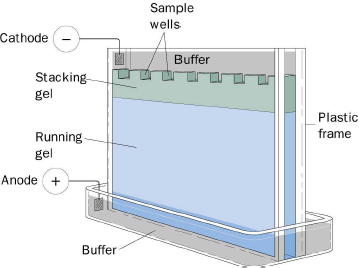
\includegraphics[width=1\textwidth]{paste_src/2023-11-13-16-00-45.png}
    \end{minipage}
  \end{figure}
\end{enumerate}


\subsection{SDS 及分子量測定}
Sodium dodecyl sulfate(SDS) 是界面活性劑,會在蛋白質分子表面均勻佈上一層負電荷,使得蛋白質電泳的結果不受馾白質自身電性影響。因此 SDS 電泳的結果只和蛋白質分子量相關。$\ce{\beta}$-mercaptoethanol(β-ME, 2-ME) 和 Dithiothreitol(DTT) 都能打斷雙硫鍵,同樣濃度下 DDT 效果較好。兩者會搭配 SDS 使用。

\subsection{蛋白質染色方法}






\section*{實驗步驟:}

\subsection*{實驗器材}



\subsection*{步驟}





\section*{實驗結果及討論:}
\subsection*{結果}

  




\subsection*{實驗數據}


\subsection*{實驗作圖}



\newpage
\subsection*{實驗討論:}




\newpage
\section*{延伸討論}





\bibliography{bibfile} 
\bibliographystyle{unsrt}
